\subsubsection{Iteration 3: Test Flight in Realistic Environment}

\paragraph{Redesign}

In the last iteration, the user finds hard to find direction in first person view, as the simple skydom environment can not delivery clear direction information.

A realistic environment can be built to solve that. With the data from \parencite{TallinnCityModel2012} and \parencite{EstonianLandBoard2020}, a city model were imported in Unity as the environment \cref{fig:tallinn}. 

This new scene gives the player a task that one should start from the Viru Gate and pilot to Tallinn Town Hall. To form a direct goal, signs of direction and game element like coins are made for guiding.

A small HUD 2D map was added for the player to clearly know one's position and his goal.

In case of missing the direction, the box collider is changed to mesh collider to support the route.

\paragraph{Enactment}

The followings are the imported map. In order to render the city in the headset, the Occlusion culling was used for cutting down the mesh render.

\begin{figure}[H]
    \caption{The Tallinn old town model (Up) and the terrain (Under) imported in Unity}\label{fig:tallinn}
    \centering
    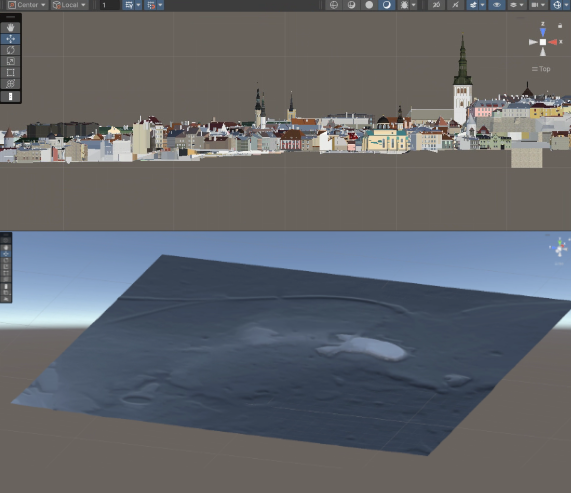
\includegraphics[width=0.8\linewidth]{img/Tallinn.png}
\end{figure}

After fine tune the skydon and the building material, the result shows as \cref{fig:realistic}.

\begin{figure}[H]
    \caption{The route (up), the final player view(bottom-left) and the coin collecting and the mesh collider (bottom-right)}\label{fig:realistic}
    \centering
    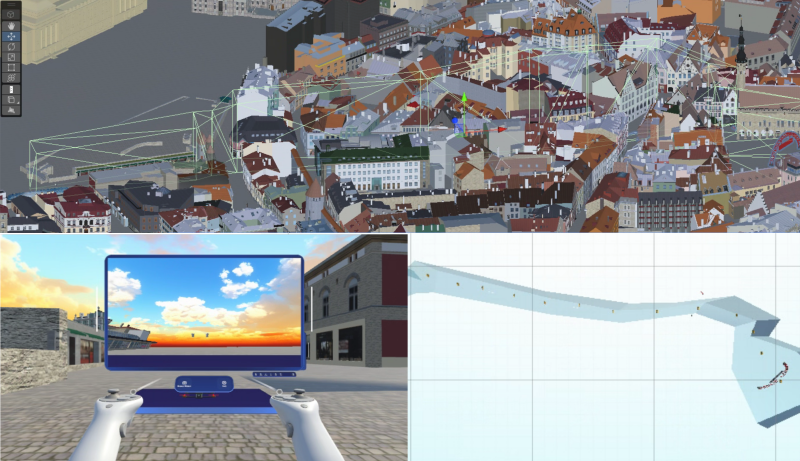
\includegraphics[width=0.8\linewidth]{img/real.png}
\end{figure}


\paragraph{Analysis}

The realistic environment gives exiting experience for the testers, some suggest that open the map for exploration which collide with the fourth stage of experiential learning, active experimentation.but the city rendering drew a performance issue, some suggest that using a white-boxed playground environment.